\chapter{Introduction and goals}
\todo{show uni dropout rates and reasons from German statistics;
point out missing knowledge about job rules; describe how it should be that less people quit uni}
At one point of every students life, they have to make a decision about the specialization of their education. This decision is mostly due when applying for a course at a higher educational institute. For students, this decision can be challenging, because it has a great impact for their future but often less information is provided by the schools or universities. This results in high drop out rates, as seen in \cite{UlrichHeublein.Juni2017}, a study about dropout rates in Germany and their reasons: \\ In total, about one third (32\%) left German universities without a degree in 2016. Most of the students quit their course because of too high requirements and difficulties in the exams (30\%). The second important reasons were a lack of motivation (17\%) and the missing of practical work and exercises (15\%). The study also pointed out that within the group of university dropouts about 56\% did not study their originally desired subject, whereas 76\% of the successfully graduated students got a degree in their desired course. On of the results of the study was that courses with an admission restriction had less dropouts than courses without. Regarding to the researches, this is because prospective students occupy more intense with their subject when they have to pass several obstacles like writing a motivation letter for applying. \\
Looking at the second and third most important reasons for a university dropout together, it is with over one third a very large group, but could be avoidable. With missing imagination and information about the profession the students are later able to work in, the endurance might not be very high. As a conclusion, motivation lacks occur and it is harder for the students to get through more theoretical parts of their studies. As well, it is also shown in the study that occupying with the subject before applying for a course results in less amounts of university dropouts. \\
The question is now: How to provide prospective students suitable information for the profession of their desired course? And more important: How is it possible to engage students in getting to know their future job roles?

One possible answer to that questions could be an internship as a entry requirement for a course. There are schools and universities which already taken this idea and put an internship on their requirement list (TODO sources). However, for prospective students, this means a high effort and a significant amount of time they have to spend on finding an internship and carrying it out. There should be a solution which is less time consuming and yet provides prospective students a real experience of their future job roles.\\
Another idea is to use the concepts and technologies of virtual reality (VR). Virtual reality describes a computer generated 3D environment which can be experienced by the users. Mostly the user is wearing a special goggle through which they are fully shielded off from the real surroundings. It is possible to get an immerse and real experience of the virtual environment, and users feel as they are actually present in the virtual world. \cite{Linowes.2015}\\
The advantages of using VR to give information about future job roles are the less costs, less time consuming and yet a nearly real experience for users. This thesis will examine the idea of a VR job role simulation for prospective students. The aim of this thesis is not only to give a theoretical research but also to develop a prototype of a VR application for prospective students. 

\section{Overview of the thesis}
This thesis will investigate the usage of VR for helping prospective students with decision making about their future profession.
The work will be limited to the information technology courses offered at Nanyang Polytechnic, a polytechnic located in Singapore. At first there will be a  research in basic VR technologie and current developments. Common problems, which occur when designing a VR application will be described as well as their solutions. Following, a storyline for the application will be designed, suitable hardware and software will be evaluated. The next step will be to implement a prototype VR application on an agile approach. This application should provide information about the different IT job roles related to the IT diploma courses at Nanyang Polytechnic.  After that the application will be tested by some test persons to get feedback. In conclusion, the whole project will be evaluated under the aspect of fulfilling the purpose of helping prospective students in understanding their future job roles.

\section{What is virtual reality?}
\todo{Definition; use; popularity; difference from AR}
According to \cite{Fuchs.2011} virtual reality is a simulated virtual world, made with hardware and software. It provides a real time user interaction and the users feel the maximum amount of immersion when experiencing the computer generated world. The virtual world is mostly provided by a head mounted display (HMD) as seen in figure \ref{fig:hmd}. This device splits the main scene into two different camera perspectives for each eye of the user. The two perspectives will then be merged into on three dimensional picture by the users brain. \\
\begin{figure}[h!]
  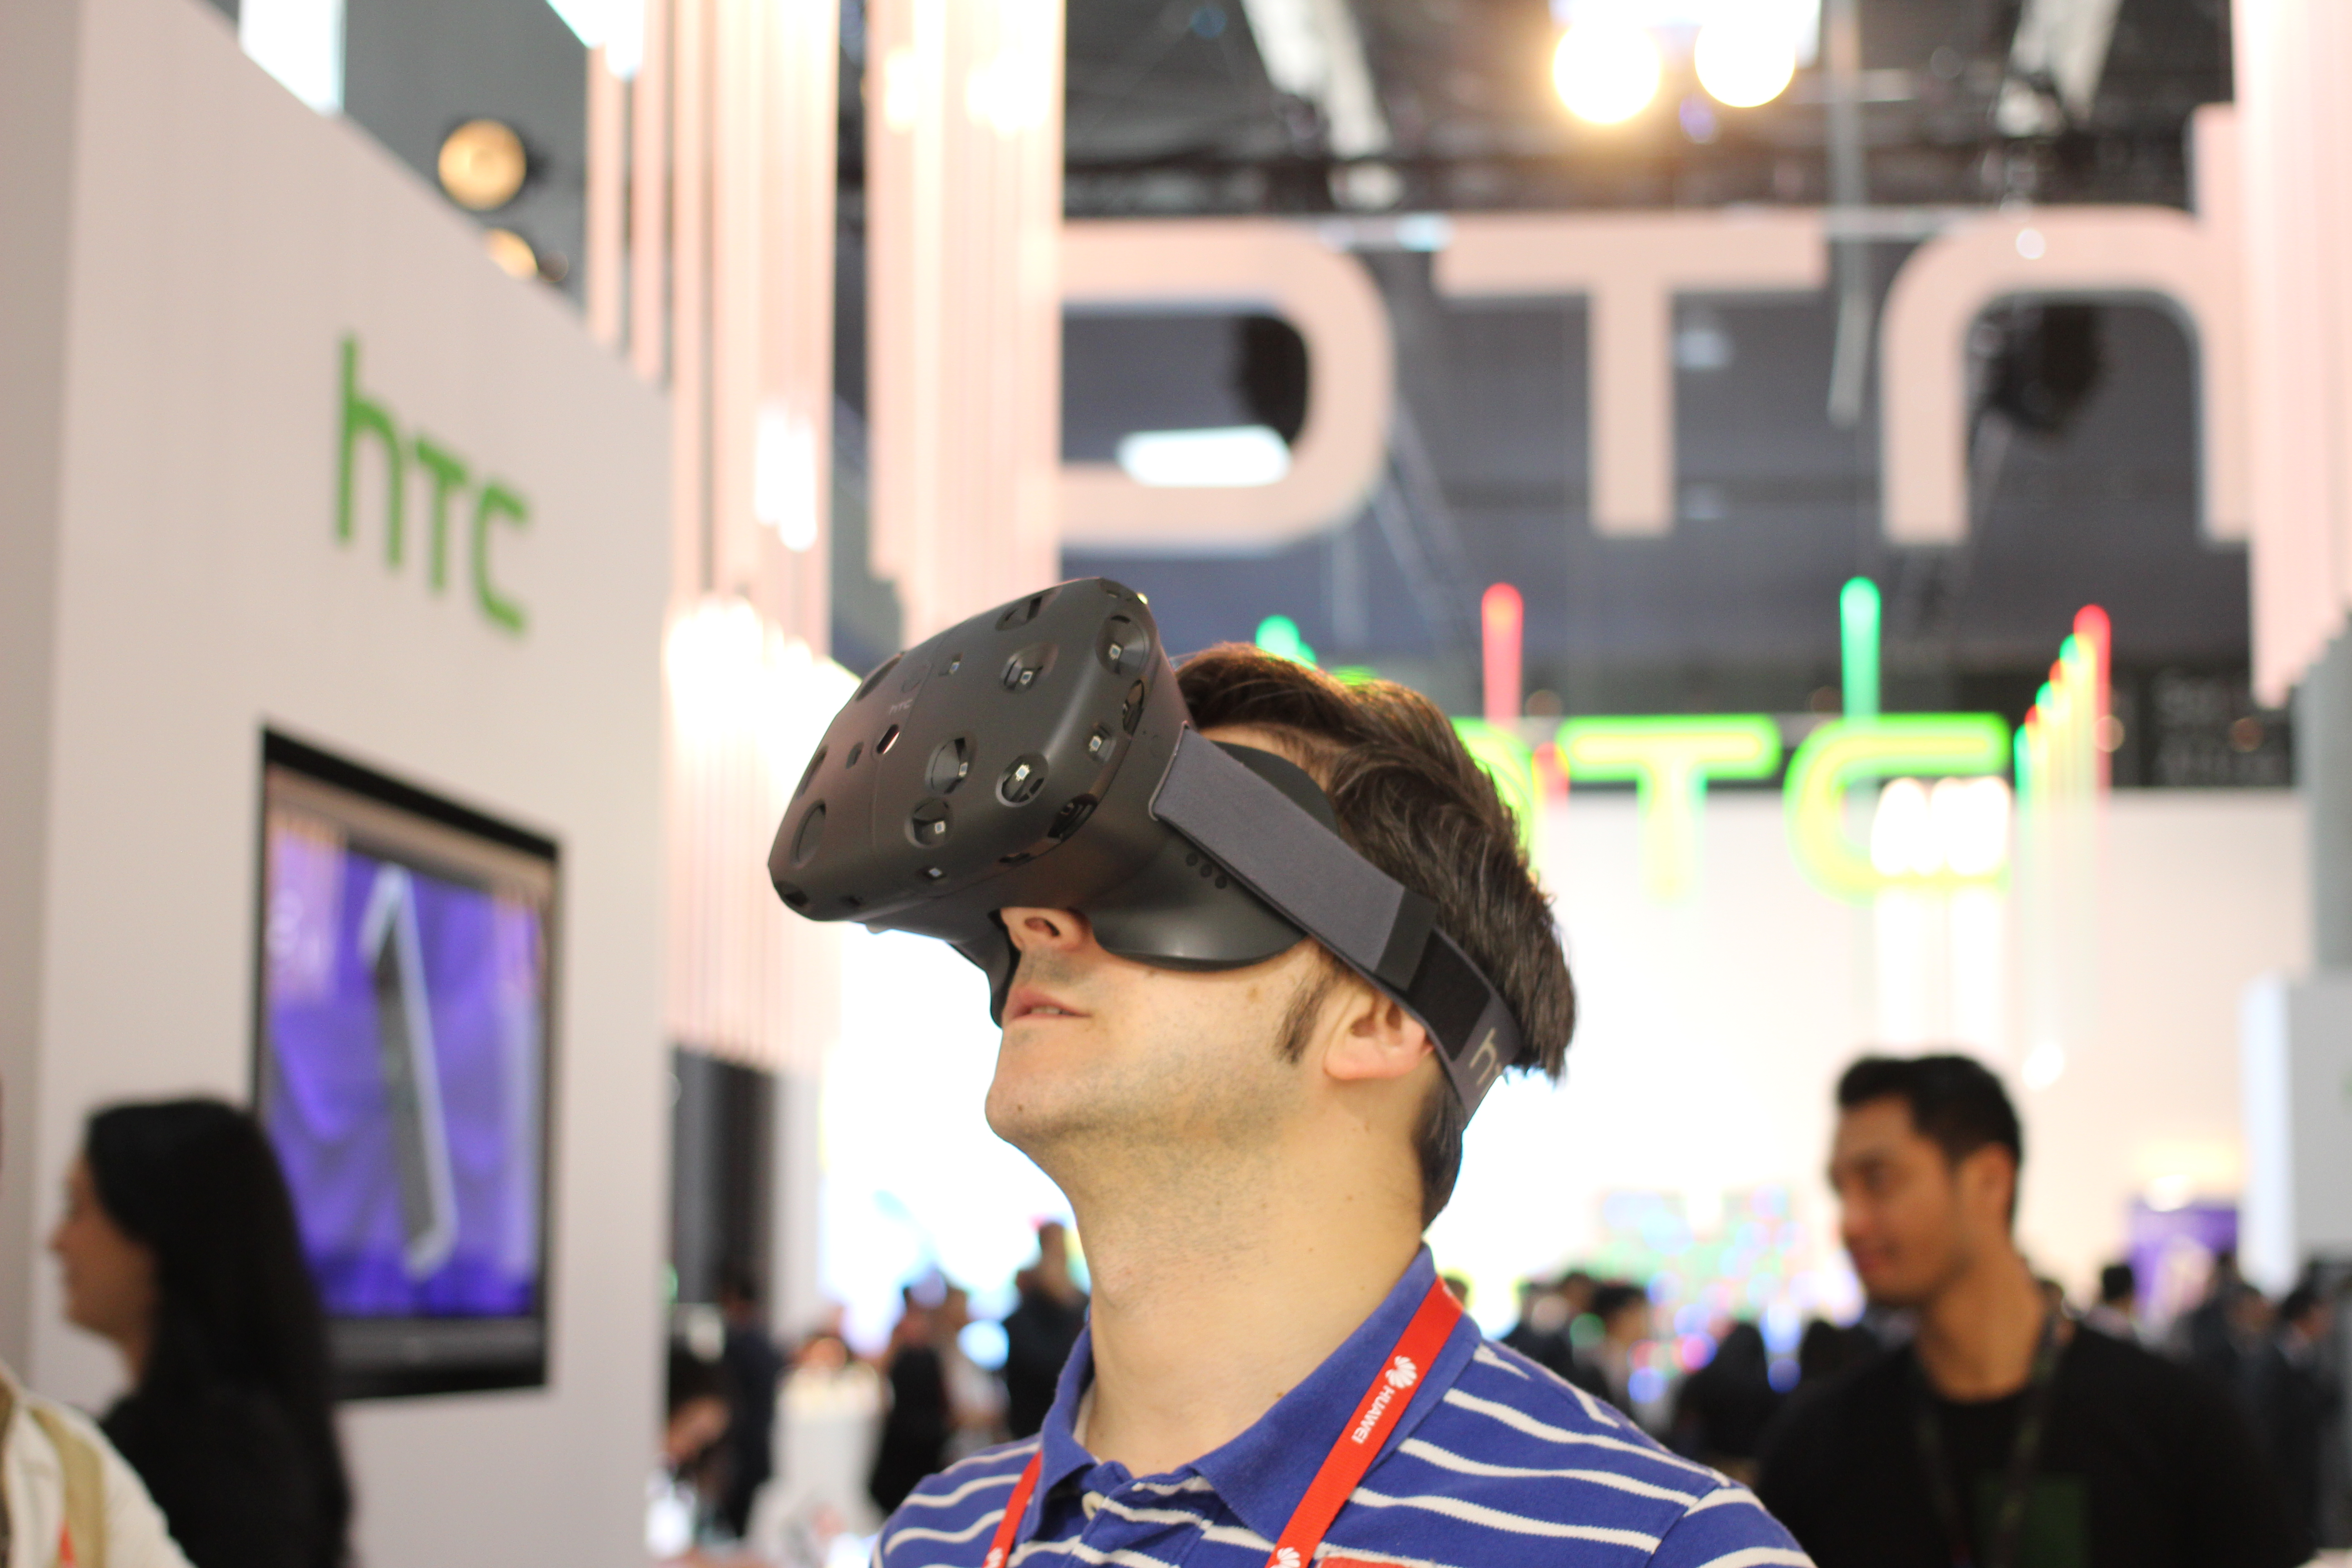
\includegraphics[width=70mm]{kapitel/HMD-example.jpg}
  \centering
  \caption{Head mounted display - by Maurizio Pesce -  \url{https://www.flickr.com/photos/pestoverde/17136177965}, CC BY 2.0, \url{https://commons.wikimedia.org/w/index.php?curid=39894108}
}
  \label{fig:hmd}
\end{figure}
The computation of the virtual world can be either done on a standalone desktop PC, on which the HMD is connected with, or directly in the HMD, for example through a mobile phone which is inside some special HMDs.\\
Despite from augmented reality (AR), virtual reallity provides a fully self-contained environment and does not interact with elements of the real world. Argumented reality on the other hand embeds virtual content into the real environments. Thereby the borders between reality and simulation become blurry. AR is a closely related technology to VR, but this thesis will focus on a virtual reality application only.\\
The usages of virtual reality are very widespread. \cite{Linowes.2015} describes a variety of different areas in which virtual reality can be used: Especially the gaming industry stands out for one of the first industries to develop VR applications and hardware devices. This is because most of the modern computer games take place in a computer generated, first person, 3d environment. It is thereby obvious to develop the games further into virtual reality applications. Lately, non-gaming VR applications are becoming more and more important. Design and architecture is a branch, where virtual reality is used to visualise prototypes in a new way to customers. In education, VR applications are used to train learners  in a nearly real environment but without the cost and danger of a real life exercise. Military training or disaster management for example are a good showcase for the usage of virtual reality in education. Another area, in which virtual reality is used, is tourism. It is possible to visit a museum without actually travelling to the place, through a virtual reality application. VR can give more immerse insights of a travelling destination and yet can be an instrument of marketing for the tourist destinations.

\section{NYP information technology courses}
This thesis will investigate the usage of virtual reality in the area of student acquisition. The aim is to help students with their decision for their diploma courses, but it is also important to make the VR experience enjoyable for prospective students.\\
The prototype application will be focused on the information technology diploma courses offered at the Nanyang Polytechnic. In the following, the environment of the school and the courses will be described.

Nanyang Polytechnic (NYP) is a polytechnic located in Ang Mo Kio, Singapore. The school offers post-secondary education for students who successfully passed the GCE O-Level examination. The O-Level examination is an annually examination mainly for students who have visited a secondary school. \cite{aboutOLevel} \\ 
It allows the students to take courses either on a junior college, a technical institute or a polytechnic. In Singapore, a polytechnic offers students a more practical and industry based education than a junior college which has a more fundamental approach. In general, students study 3 years at a polytechnic until they get their diploma. After getting a diploma, students can continue their education at a university but they can also start to work in the industry. \cite{schoolSystem}\\
NYP offers a wide range of courses in different fields. One of the fields is information technology (IT). In the following the courses will be introduced briefly: \cite{nypCourses}

\paragraph{Information Technology}
This course offers students a broad range of the different fields in information technology. It focuses on an interdisciplinary education. By finishing the course, students are prepared to work in different areas, most commonly in software engineering. During the first year, the fundamental topics of information technology are educated. The second year deepens the knowledge in application programming, database management, software engineering, algorithms and several other topics. The third year will be for specialization. The students can choose elective courses in the fields of artificial intelligence, enterprise cloud computing, geospatial and mobile innovation and cybersecurity. As in all courses offered at the school of information technology, there is one practical industry project and an internship in the third year as well.

\paragraph{Infocomm and Security}
This course covers topics in IT infrastructure, network engineering and security and the internet of things (IoT). Students learn how to program, but also how to secure applications in a connected environment. They also learn about managing connected infrastructures. During the first year there are basic classes in developing and infocomm to get a grounded knowledge in information technology. The second year will deepen the knowledge of network engineering, programming, and IT service management. There will be a practical IoT project for the students as well.
In the third year there will be several elective courses in the areas of system and network security, enterprise infrastructure and infocomm solutions.

\paragraph{Cybersecurity and Digital Forensics}
The cybersecurity and digital forensic course focuses on IT security. This includes securing systems and data for unauthorized access as well as tracing criminals in case a security incident happened. After graduating, students can work as security analysts, network penetration tester, security engineer and similar jobs. During the first year students learn fundamental IT skills. The second year offers classes in forensics, network security, operating systems, security standards and more. Students will also complete an applications security and an infosecurity project.
The last year offers specialization in the topics cybersecurity track and cyber forensics track. It is possible to choose crossdisciplinary classes from other IT courses.

\paragraph{Business Intelligence and Analytics}
The business intelligence and analytics course teaches analytics and interpretation of massive amounts of data. Therefore big data technologies, as well as artificial intelligence is needed. After graduating, it is possible to work as a data or business analyst, a social media strategist or a digital marketing executive. During the first year student will gain basic IT and business statistic knowledge. The second year offers classes in big data management, digital marketing, predictive modelling and similar topics. Students participate on a big data and a business analytics project.
During the third year, students will do a data science project and can choose between several elective classes.

\paragraph{Business and Financial Technology}
This course focuses on information technology in the financial and business sector. After getting a diploma, students can work as IT or financial consultants, financial application specialists or business and financial analysts. From the beginning the focus lies on connecting business and financial topics with information technology. Therefore, in the first year students learn about economics, accounting and consumer banking as well as about basic programming skills. During the second year this knowledge is deepened through classes like software engineering or financial management. Besides the elective classes, the industry project and internship, students in the third year also collaborate in a fintech innovation project.

\section{Advantages of VR for prospective students}
\todo{Explain why VR and future professions work well together, point out immersion of VR, name examples of similar VR projects}
The last chapter summed up the information about the information technology diploma courses in textual representation. Therefore the question occurs, why it is necessary to develop a VR application if the required information can be distributed to prospective students through other media as well. Or to put it in other words: Can prospective students profit from experiencing their future profession through a virtual reality application? \\
The thesis will take a close look at two different groups: Prospective students, using virtual reality to inform themselves about their future job roles and prospective students, using traditional media (e.g. flyers, websites) as resource.
The predicted outcome of this research is that there will be a difference between those groups. Students using the virtual reality application will have a clearer understanding of their profession and will be able to remember the provided information easier. They will get a more comprehensive idea of the different job roles in IT  than the group with the traditional media for informing. \\

Despite the area of information keeping, virtual reality is a currently researched topic of information technology. Students are able to use technologies, which they later get into closer touch with. The idea is to arouse interest in the technology behind virtual reality and to make the students want to develop their own application. Prospective students can profit as well from the cheaper and less time consuming approach in getting to know a future job role, compared to an internship. 
